\chapter{} \label{Chap1}
\section{Introduction}
In today's interconnected world, networks are critical components of many complex systems, including financial markets\cite{tumminello2010correlation}\cite{bonanno2004networks}, transportation systems, and social networks. The interconnectivity of these systems also creates vulnerabilities that can result in systemic risk, which can have far-reaching consequences. This report first analysed the distributional properties of balance sheet and topological properties of a specific bank network, and then researched the models related to systemic risk in networks. In particular, this report explores how the default of a bank can impact the broader banking system, using four different simulation models under a series of stress test. By analyzing the potential effects of a bank default on the entire banking system, this report aims to provide valuable insights into how to identify and mitigate systemic risk in networks. Ultimately, this report highlights the importance of understanding and managing systemic risk to ensure the stability and resilience of our interconnected systems.


\section{Task 1: Distributional and Topological Properties}
\subsection{Distributional Properties of Balance Sheet}
\begin{table}[H]
    \caption[table]{Distributional Properties of Balance Sheet}
    \vspace{0.5em}\centering
    \begin{tabular}{cccccc}
        \toprule[1.5pt]
                              &Mean        &Median      &Standard Deviation &Skewness  &Kurtosis\\
        \midrule[1pt]                            
        Interbank Asset       &16729955.8  & 2341851.6  & 37065062.5        &3.2       &11.0\\
        External Asset        &66997512.9  & 7318800.0  &201000355.9        & 7.6      &72.7\\
        Interbank Liabilities &16729955.8  & 1828090.8  & 50196967.3        &7.6       &72.7\\
        External Liabilities  &60115606.6  &7602735.32  &166311812.5        &6.4       &53.3\\
        Equity                & 6881906.3  &  515310.0  & 19752366.3        &5.3       &34.1\\
        \bottomrule[1.5pt]
    \end{tabular}
\end{table}

\begin{figure}[H]
    \centering
    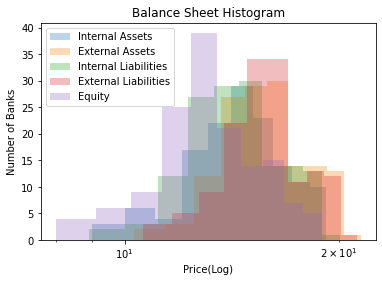
\includegraphics[width = 0.4\linewidth]{Balance Sheet Histogram.png}
    \caption{Balance Sheet Histogram}\label{fig:Balance Sheet Histogram}
\end{figure}

Balance sheets are important financial statements\cite{williams2008financial} that provide a snapshot of a company's financial health. In addition to the actual values reported on a balance sheet, there are several distributional properties that can help to provide insights into the underlying financial performance of a company. These properties include the mean, median, standard deviation, skewness, and kurtosis.

The mean, or average, is a commonly used measure of central tendency that provides an indication of the typical value of a distribution. For the given balance sheet data, the mean Interbank Asset is 16729955.8, which is relatively low compared to the other categories. This suggests that the company may have a smaller amount of interbank assets compared to other types of assets. The mean External Asset is much higher at 66997512.9, indicating that external assets represent a significant portion of the company's overall assets. The mean Interbank Liabilities is the same as the mean Interbank Assets, indicating that the company may have an equal amount of interbank assets and liabilities. The mean External Liabilities is 60115606.6, indicating that external liabilities represent a significant portion of the company's overall liabilities. Finally, the mean Equity is relatively low at 6881906.3, suggesting that the company may have a small amount of equity relative to its overall assets and liabilities.

The median is another measure of central tendency that provides an indication of the value that separates the top 50\% of a distribution from the bottom 50\%. The median values for each of the balance sheet categories are generally lower than the mean values, indicating that the distributions are skewed to the right. For example, the median Interbank Asset is 2341851.6, which is much lower than the mean value of 16729955.8. This suggests that there may be a few large interbank assets that are driving up the mean value. The median External Asset is also much lower than the mean at 7318800.0, indicating that there are likely a few large external assets that are driving up the mean value. The median values for Interbank Liabilities, External Liabilities, and Equity are all lower than the mean values, indicating that the distributions are skewed to the right.

The standard deviation is a measure of how spread out a distribution is from its mean value\cite{bland1996statistics}. For the given balance sheet data, the standard deviation is relatively high for all categories, indicating that the distributions are fairly wide. For example, the standard deviation for External Asset is 201000355.9, which is much higher than the mean value of 66997512.9. This indicates that there is a large amount of variability in the external assets held by the company.

Skewness is a measure of how asymmetrical a distribution is\cite{bowley1920elements}. A positive skewness value indicates that the distribution is skewed to the right, while a negative skewness value indicates that the distribution is skewed to the left. For the given balance sheet data, all categories have positive skewness values, indicating that the distributions are skewed to the right. The highest skewness value is for External Asset at 7.6, suggesting that there may be a few very large external assets that are driving up the mean value.

Kurtosis is a measure of how peaked or flat a distribution is relative to a normal distribution\cite{pearson1905fehlergesetz}. A positive kurtosis value indicates that the distribution is more peaked than a normal distribution, while a negative kurtosis value indicates that the distribution is more flat than a normal distribution. For the given balance sheet data, all categories have positive kurtosis values, indicating that the distributions are more peaked than a normal distribution. The highest kurtosis value is for External Asset at 72.7, suggesting that there may be a few extreme values that are driving up the peak.

\subsection{Topological Properties of Network}

\begin{figure}[H]
    \centering
    \begin{minipage}{0.49\textwidth}
    \centering
    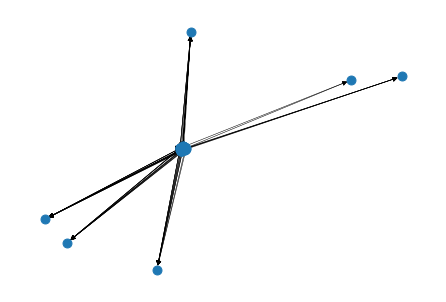
\includegraphics[width = \linewidth]{Graph Topology.png}
    \caption{Normal Layout}\label{fig:Degree Distribution}
    \end{minipage}
    \centering
    \begin{minipage}{0.49\textwidth}
    \centering
    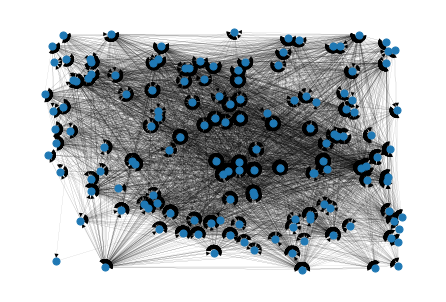
\includegraphics[width = \linewidth]{Graph Topology with Random Layout.png}
    \caption{Random Layout}\label{fig:Degree Distribution with Random Layout}
    \end{minipage}
    \caption{Degree Distribution}
\end{figure}

Firstly, the natural topological graph of the interbank exposure network is presented in \ref{fig:Degree Distribution}, as well as the random position topological graph of the interbank exposure network is presented in \ref{fig:Degree Distribution with Random Layout}

The topological properties of a network are crucial for understanding its behavior and dynamics. Next, the topological properties of the network are described as follows, which involves 4 key properties: degree distribution, centrality, clustering and assortativity.

\subsubsection{Degree Distribution}
Degree distribution is a fundamental topological property of networks, which describes the probability distribution of the number of links (or edges) that each node (or vertex) has in the network. The degree distribution for a network is defined as the probability that a randomly selected node has degree k, that is, the number of nodes with degree k over the total number of nodes. Mathematically, if $G$ is a network with $N$ nodes, and $k_i$ is the degree (i.e., the number of edges) of node $i$, then the degree distribution is defined as $P(k)$, where $P(k)$ is the probability that a randomly selected node has degree $k$ in the network $G$. In other words, $P(k)$ measures the frequency of nodes with degree $k$ in $G$.

\[
    P(k) = \frac{N_k}{N}
\]

\begin{figure}[H]
    \centering
    \begin{minipage}{0.49\textwidth}
    \centering
    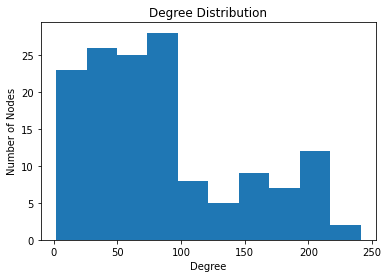
\includegraphics[width = \linewidth]{Degree Distribution1.png}
    \caption{Degree Distribution}\label{fig:Degree Distribution1}
    \end{minipage}
    \centering
    \begin{minipage}{0.49\textwidth}
    \centering
    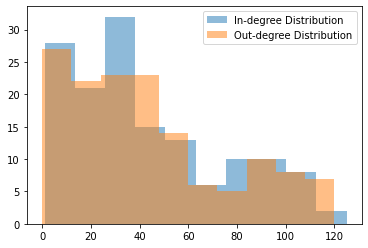
\includegraphics[width = \linewidth]{Degree Distribution2.png}
    \caption{In and Out Degree Distribution}\label{fig:Degree Distribution2}
    \end{minipage}
    \caption{Degree Distribution}
\end{figure}

In \ref{fig:Degree Distribution1}, for each degree k on the X-axis, the Y-axis represents the number of nodes which have degree k, i.e., Nk. It can be observed that over two thirds of 145 nodes (banks) have a degree below 100, with the rest one third having a degree from 100 to 250, thus the systematic risk cannot be ignored (the maximum degree could be $145*2=290$).

In \ref{fig:Degree Distribution2}, the degree is broken down into two categories: the blue area is the in-degree distribution while the yellow represents the out-degree distribution. Similarly, many banks have an in- or out-degree below 50, while there are still some having a degree above that.

\begin{figure}[H]
    \centering
    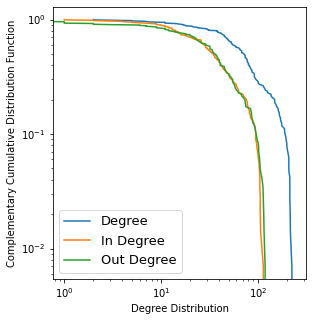
\includegraphics[width = 0.32\linewidth]{In and Out Degree Distribution CCDF Log Plot.png}
    \caption{In and Out Degree Distribution CCDF Log Plot}\label{fig:In and Out Degree Distribution CCDF Log Plot}
\end{figure}

One of the most commonly observed degree distributions in real-world networks is the power-law distribution, also known as the scale-free distribution, which is defined as $P(k)\varpropto k^{-\gamma}$, where $\gamma$ is a positive exponent that characterizes the network's connectivity. This means that there are a few nodes with very high degree (known as "hubs"), and many nodes with low degree, resulting in a heavy-tailed distribution. Power-law degree distributions have been observed in many natural and man-made networks, such as the World Wide Web, social networks, and citation networks.

\ref{fig:In and Out Degree Distribution CCDF Log Plot} is the complementary cumulative distribution function of in degree and out degree which were plotted in log-log scale. It indicats that the distribution of degree in this network is not the power-law distribution because it does not have power-law tailed.

\subsubsection{Centrality}
Centrality is another important topological property of networks, which characterizes the importance of nodes in the network based on their connectivity patterns. There are several types of centrality measures, including degree centrality, betweenness centrality, and eigenvector centrality.

Degree centrality\cite{freeman2002centrality} is the simplest and most intuitive centrality measure, which is based on the number of edges incident to a node. Mathematically, if $k_i$ is the degree of node $i$, then the degree centrality of node $i$ is defined as $C_i = k_i/(N-1)$, where $N$ is the total number of nodes in the network. This means that $C_i$ measures the fraction of nodes in the network that are directly connected to node $i$. Nodes with high degree centrality are often considered as important hubs or gatekeepers in the network.

\begin{figure}[H]
    \centering
    \begin{minipage}{0.49\textwidth}
    \centering
    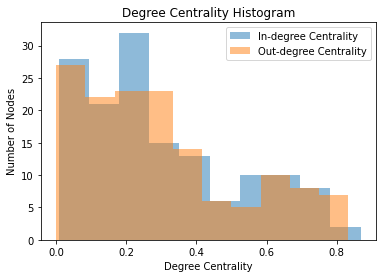
\includegraphics[width = \linewidth]{Degree Centrality Histogram.png}
    \caption{Histogram}\label{fig:Degree Centrality Histogram}
    \end{minipage}
    \centering
    \begin{minipage}{0.49\textwidth}
    \centering
    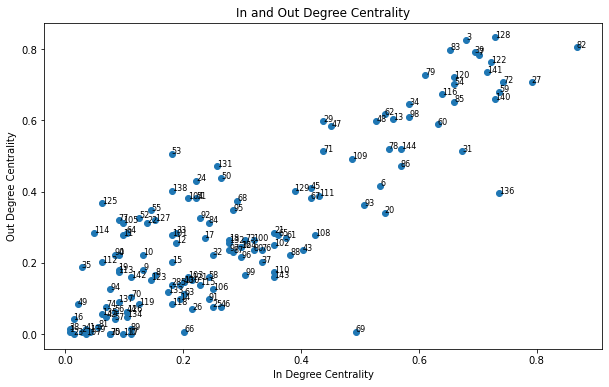
\includegraphics[width = \linewidth]{Degree Centrality Scatter Plot.png}
    \caption{Scatter Plot}\label{fig:Degree Centrality Scatter Plot}
    \end{minipage}
    \caption{Degree Centrality}
\end{figure}

Apart from the degree centrality, there are other centrality measures containing more information about the overall network other than just about the neighbourhood of a node.
\begin{figure}[H]
    \centering
    \begin{minipage}{0.49\textwidth}
    \centering
    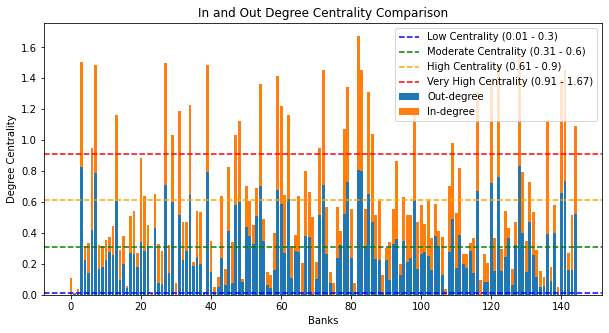
\includegraphics[width = \linewidth]{Centrality Comparison.png}
    \caption{Centrality Comparison}\label{fig:Centrality Comparison}
    \end{minipage}
    \centering
    \begin{minipage}{0.49\textwidth}
    \centering
    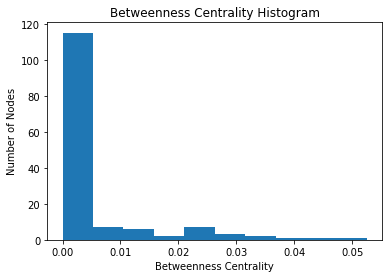
\includegraphics[width = \linewidth]{Betweenness Centrality Histogram.png}
    \caption{Betweenness Centrality Histogram}\label{fig:Betweenness Centrality Histogram}
    \end{minipage}
\end{figure}


The betweenness centrality of a node is the number of shortest paths between any two nodes that pass through this node. Mathematically, if $\sigma_{s,t}$ is the total number of shortest paths between nodes $s$ and $t$ in the network, and $\sigma_{s,t}(i)$ is the number of shortest paths that pass through node $i$, then the betweenness centrality of node $i$ is defined as $B_i = \sum_{s,t} \frac{\sigma_{s,t}(i)}{\sigma_{s,t}}$, where the sum is taken over all pairs of nodes $s$ and $t$ in the network. This means that $B_i$ measures the fraction of shortest paths in the network that pass through node $i$. Nodes with high betweenness centrality are often considered as important brokers or connectors in the network.

\[
    B_i = \sum_{k > j\neq i}\frac{\text{\# of geodesic paths between kand j passing through i}}{\text{\# of geodesic paths between kand j}}
\]

\begin{figure}[H]
    \centering
    \begin{minipage}{0.49\textwidth}
    \centering
    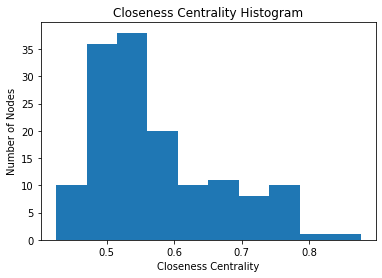
\includegraphics[width = \linewidth]{Closeness Centrality Histogram.png}
    \caption{Closeness Centrality Histogram}\label{fig:Closeness Centrality Histogram}
    \end{minipage}
    \centering
    \begin{minipage}{0.49\textwidth}
    \centering
    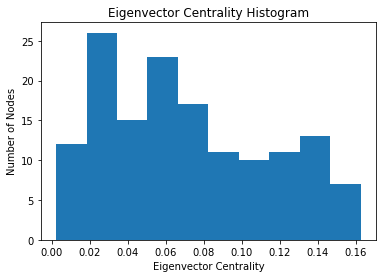
\includegraphics[width = \linewidth]{Eigenvector Centrality Histogram.png}
    \caption{Eigenvector Centrality Histogram}\label{fig:Eigenvector Centrality Histogram}
    \end{minipage}
\end{figure}
Eigenvector centrality\cite{zaki2014data} is a centrality measure that takes into account the connectivity of a node's neighbors. Mathematically, if $A$ is the adjacency matrix of the network, and $v_i$ is the eigenvector corresponding to the largest eigenvalue $\lambda_{max}$ of $A$, then the eigenvector centrality of node $i$ is defined as $E_i = v_i(i)/\sigma_j v_i(j)$, where $v_i(j)$ is the $j^\text{th}$ component of $v_i$. This means that $E_i$ measures the extent to which node $i$ is connected to other nodes with high centrality in the network. Nodes with high eigenvector centrality are often considered as important influencers or trendsetters in the network.

\subsubsection{Clustering}
Clustering\cite{holland1971transitivity} is a measure of the degree to which nodes in a network tend to form local clusters or communities. Mathematically, if $G$ is a network with $N$ nodes, and $C(i)$ is the number of triangles (i.e., three-node subgraphs) that include node $i$, then the clustering coefficient of node $i$ is defined as

\[
    C_i = \frac{e_i}{k_i(k_i - 1)/2}
\]

Where $e_i$ is the number of actual links between neighbours of the node $i$, and $k_i*(k_i-1)/2$ is the number of possible links between neighbours of the node $i$. The clustering coefficient is a measure of the tendency of forming cliques in the neighbourhood of a node.

\begin{figure}[H]
    \centering
    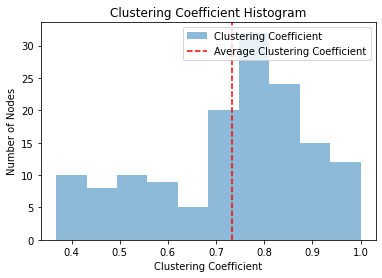
\includegraphics[width = 0.32\linewidth]{Clustering Coefficient Histogram.png}
    \caption{Clustering Coefficient Histogram}\label{fig:Clustering Coefficient Histogram}
\end{figure}
\ref*{fig:Clustering Coefficient Histogram} is a distribution of clustering coefficients with an average around 0.73. Two thirds of 145 banks have a clustering coefficient above 0.7, suggesting that there is a strong tendency for these banks to form cliques and they will be affected by shocks together.

\subsubsection{Assortativity}
The assortativity coefficient is a measure of the tendency of nodes to be connected with nodes with similar degree. If the coefficient is positive, high degree nodes will tend to be connected with high degree nodes; but if it is negative (i.e., disassortativity), high degree nodes will tend to be connected with low degree nodes.

\begin{lstlisting}[language=python]
    The assortativity coefficient of G = -0.3882919829621765
\end{lstlisting}

The assortativity coefficient of this interbank exposure network is calculated, which is a negative value -0.388292, indicating that the tendency is more similar to a technological network rather than a social network.

\section{Task 2: Stress Tests:}
The Furfine algorithm\cite{furfine1999pricing} is a widely used method for analyzing interbank defaults in a network of banks. It is named after its creator, Craig Furfine, and is based on the simple idea of tracking the state of each bank in the network and updating their equity values as shocks occur.

The algorithm begins by defining the state of each bank in the network as either running or in default. A shock is then applied to the system, such as a bank defaulting or the external assets of a group of banks being devalued. This shock causes changes in the assets and liabilities of each bank in the network.

Each bank then updates the value of its equity using the formula equity = assets - liabilities. If this value falls below zero, the bank is considered to be in default. The state of each bank is then updated accordingly.

If any new defaults occur as a result of the shock, the algorithm returns to step three and updates the equity values of each bank again. This process continues until there are no more new defaults.

The Furfine algorithm is particularly useful for analyzing interbank defaults in a network because it takes into account the interconnectedness of the banks in the network. It recognizes that the failure of one bank can have a cascading effect on other banks in the network, potentially leading to a systemic crisis.

By tracking the state of each bank and updating their equity values in response to shocks, the algorithm allows analysts to simulate the effects of various shocks on the network and to identify the banks that are most vulnerable to default.

\subsection{Scenario 2.1: One bank default}
Firstly, I analyzed a scenario in which a bank defaults initially and simulated the network contagion using the Furfine algorithm. 

\begin{figure}[H]
    \centering
    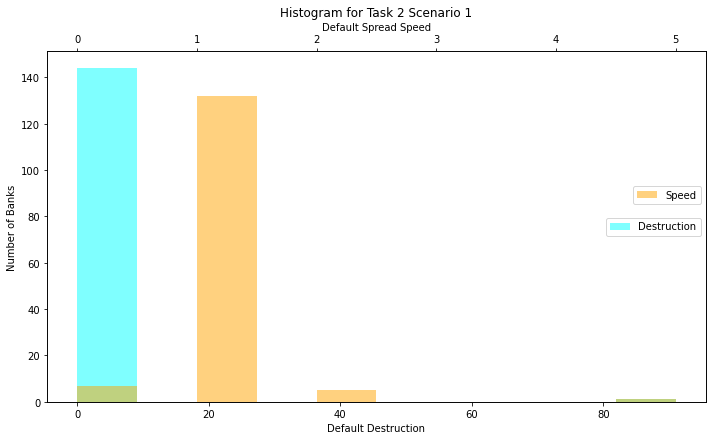
\includegraphics[width = 0.5\linewidth]{Task 2 Scenario 1.png}
    \caption{Task 2 Scenario 1}\label{fig:Task 2 Scenario 1}
\end{figure}

\begin{lstlisting}[language=python]
    The bank 82 has the biggest destruction 91
    The bank 82 has the slowest default spread speed 5
\end{lstlisting}

The results indicated that the contagion spread at a similar speed (<2 rounds) regardless of which bank was the initial defaulter. Moreover, the final outcome was the same, with most banks defaulting as a result of the shock.

\subsection{Scenario 2.2: The external assets of a group of banks are devalued}

To account for different scenarios, I analyzed the impact of a asset devalued by external reason and used the Furfine algorithm to simulate network contagion. 

\begin{figure}[H]
    \centering
    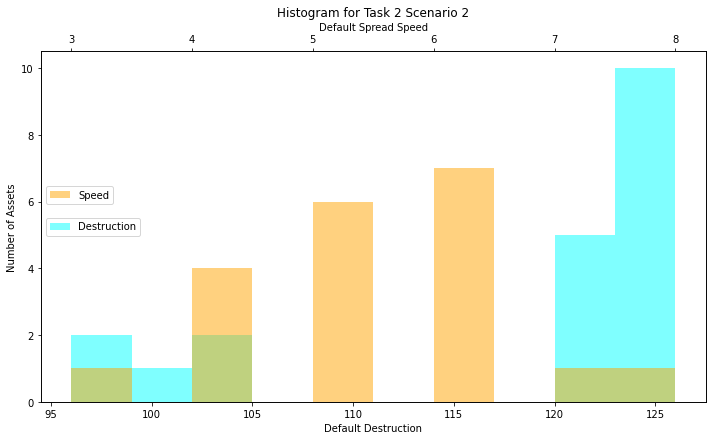
\includegraphics[width = 0.5\linewidth]{Task 2 Scenario 2.png}
    \caption{Task 2 Scenario 2}\label{fig:Task 2 Scenario 2}
\end{figure}

\begin{lstlisting}[language=python]
    The bank 8 has the biggest destruction 126
    The bank 19 has the slowest default spread speed 8
\end{lstlisting}

The results showed that the contagion speed much lower (most 4-6 rounds) until finish. However, the outcome of the destruction was very unlucky, with most banks defaulting as a result of the shock.

\section{Task 3}



\subsection{Scenario 3.1: One bank default + Linear devaluation of asset by fire-sale}
To enhance the validity of the model, I incorporated a liability default threshold (a = 0.3) to the assets devalued by the fire-sale. I maintained the same initial assumptions, with either one bank default or one asset devalued to 0. 
\begin{figure}[H]
    \centering
    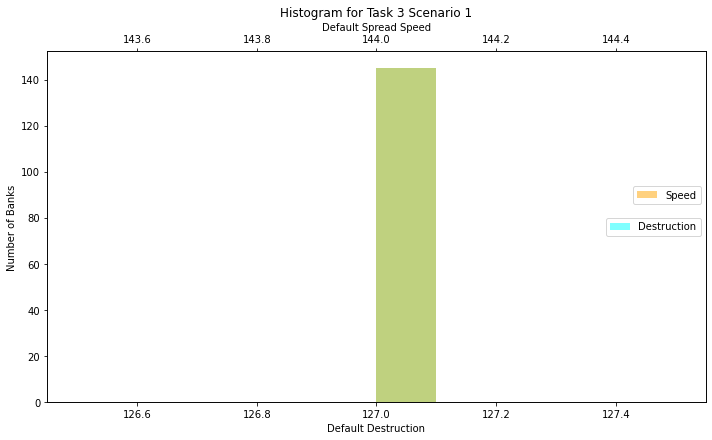
\includegraphics[width = 0.5\linewidth]{Task 3 Scenario 1.png}
    \caption{Task 3 Scenario 1}\label{fig:Task 3 Scenario 1}
\end{figure}

\begin{lstlisting}[language=python]
    The bank 0 has the biggest destruction 127
    The bank 0 has the slowest default spread speed 144
\end{lstlisting}

The results indicated that all banks eventually defaulted in 144 rounds, consistent with the previous outcomes. This modification provided a more accurate reflection of real-world scenarios, where banks have varying degrees of liability and may default at different thresholds, leading to more realistic simulations of network contagion.

\subsection{Scenario 3.2: External assets devalued + Linear devaluation of asset by fire-sale}
In the final scenario, the market impact parameter (a = 0.3) was consistent with the previous model, but different assets exhibited slightly varying outcomes. Although the contagion spread at the same speed of 144 rounds, the destruction was a tiny different across assets, ranging from 126 to 134. The most frequent outcome was around 130, indicating that the network was stable and converged to a consistent outcome. This suggests that the model was effective in capturing the dynamics of interbank contagion and can serve as a useful tool for assessing the stability of financial systems.
\begin{figure}[H]
    \centering
    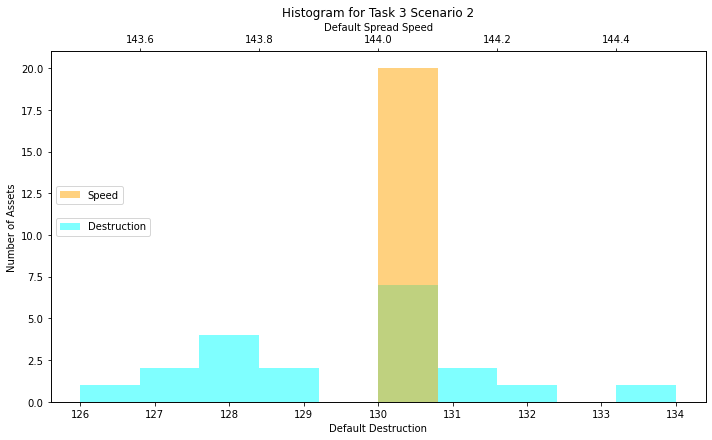
\includegraphics[width = 0.5\linewidth]{Task 3 Scenario 2.png}
    \caption{Task 3 Scenario 2}\label{fig:Task 3 Scenario 2}
\end{figure}

\begin{lstlisting}[language=python]
    The bank 18 has the biggest destruction 134
    The bank 0 has the slowest default spread speed 144
\end{lstlisting}

\section{Discussion and Conclusion}


\subsection{Interpretation of Results}
One of the strengths of the Furfine algorithm is its simplicity. It is relatively easy to implement and can be used to analyze networks of varying sizes and complexity. The algorithm also allows for the inclusion of a variety of shock scenarios, which can help analysts to better understand the potential impact of different types of shocks on the network. Simulating the effects of a shock is a straightforward process, as the model is able to accurately capture both the speed and magnitude of the resulting contagion.

Besides the simplicity, the Furfine model also offers several other advantages:

Realistic assumptions: The model makes realistic assumptions about the behavior of banks, including the fact that they will default if their equity falls below zero.

Flexible: The model can be adapted to incorporate various types of shocks and different network structures, which allows for a more nuanced understanding of the dynamics of interbank contagion.

Captures the role of interbank linkages: The model explicitly captures the role of interbank linkages in spreading contagion, which is a critical factor in understanding systemic risk in financial systems.

Quantitative analysis: The model allows for quantitative analysis of the effects of different shocks on the network, which can inform policy decisions and risk management strategies.

\subsection{Limitations and Further Challenges}

However, the algorithm does have some limitations. For example, it assumes that all banks in the network behave in the same way, which may not be the case in reality. It also does not take into account any potential government intervention or regulatory actions that could mitigate the effects of a shock.

Despite these limitations, the Furfine algorithm remains a valuable tool for analyzing interbank defaults in a network of banks. Its simplicity and flexibility make it a useful starting point for understanding the potential impact of shocks on the banking system, and it can be a valuable tool for regulators, policymakers, and analysts alike.
